% Blatt 1 — Gespraechsteil
% Kompilieren mit: lualatex gespraech.tex
\documentclass[11pt,a4paper,DIV=12]{scrartcl}
% Gemeinsame Praeambel fuer alle Blaetter.
% Einbinden mit % Gemeinsame Praeambel fuer alle Blaetter.
% Einbinden mit % Gemeinsame Praeambel fuer alle Blaetter.
% Einbinden mit \input{../../stil.tex} — Pfad ist relativ zum Kompilierordner.
% Kompiliert wird mit lualatex (wegen luatexja).

\usepackage[ngerman]{babel}
\usepackage[haranoaji]{luatexja-preset}
\usepackage{luatexja-ruby}
\usepackage{booktabs}
\usepackage{array}
\usepackage{xcolor}
\usepackage[most]{tcolorbox}
\usepackage{enumitem}
\usepackage{microtype}
\usepackage{graphicx}
\usepackage{wrapfig}
\usepackage{multicol}
\usepackage{amssymb}
\usepackage{needspace}

% Gedankenstriche als LATEINISCHE Zeichen behandeln.
% luatexja haelt sie sonst fuer Japanisch — und weil japanische Zeichen
% keine Leerzeichen brauchen, frisst es den Zeilenumbruch danach:
% "Nomen —und wenn" statt "Nomen — und wenn".
\ltjdefcharrange{100}{"2013,"2014}
\ltjsetparameter{jacharrange={-100}}
\graphicspath{{../../bilder/}}

\definecolor{akzent}{HTML}{1F4E79}
\definecolor{implizit}{HTML}{1B7A43}
\definecolor{explizit}{HTML}{B3541E}
\definecolor{hell}{HTML}{F4F6F8}

\addtokomafont{disposition}{\color{akzent}}
\setkomafont{title}{\color{akzent}\bfseries}

\newcommand{\impl}{\textcolor{implizit}{\textbf{implizit}}}
\newcommand{\expl}{\textcolor{explizit}{\textbf{explizit}}}
\newcommand{\jterm}[2]{\ruby{#1}{#2}}

% Deutsche Anfuehrungszeichen: babel-Befehle statt Unicode.
% Sonst zwei Probleme: ASCII-" ist bei ngerman ein Umlaut-Shorthand
% ("o -> oe), und luatexja haelt Unicode-Quotes fuer Japanisch und
% setzt Abstand drumrum.
\newcommand{\zitat}[1]{\glqq #1\grqq{}}

% Schreiblinie fuer Antworten
\newcommand{\lin}[1][4cm]{\rule[-0.5em]{#1}{0.4pt}}

\newtcolorbox{merke}[1][]{
  enhanced, colback=hell, colframe=akzent,
  boxrule=0pt, leftrule=3pt, arc=0pt, outer arc=0pt,
  left=8pt, right=8pt, top=6pt, bottom=6pt,
  #1
}
 — Pfad ist relativ zum Kompilierordner.
% Kompiliert wird mit lualatex (wegen luatexja).

\usepackage[ngerman]{babel}
\usepackage[haranoaji]{luatexja-preset}
\usepackage{luatexja-ruby}
\usepackage{booktabs}
\usepackage{array}
\usepackage{xcolor}
\usepackage[most]{tcolorbox}
\usepackage{enumitem}
\usepackage{microtype}
\usepackage{graphicx}
\usepackage{wrapfig}
\usepackage{multicol}
\usepackage{amssymb}
\usepackage{needspace}

% Gedankenstriche als LATEINISCHE Zeichen behandeln.
% luatexja haelt sie sonst fuer Japanisch — und weil japanische Zeichen
% keine Leerzeichen brauchen, frisst es den Zeilenumbruch danach:
% "Nomen —und wenn" statt "Nomen — und wenn".
\ltjdefcharrange{100}{"2013,"2014}
\ltjsetparameter{jacharrange={-100}}
\graphicspath{{../../bilder/}}

\definecolor{akzent}{HTML}{1F4E79}
\definecolor{implizit}{HTML}{1B7A43}
\definecolor{explizit}{HTML}{B3541E}
\definecolor{hell}{HTML}{F4F6F8}

\addtokomafont{disposition}{\color{akzent}}
\setkomafont{title}{\color{akzent}\bfseries}

\newcommand{\impl}{\textcolor{implizit}{\textbf{implizit}}}
\newcommand{\expl}{\textcolor{explizit}{\textbf{explizit}}}
\newcommand{\jterm}[2]{\ruby{#1}{#2}}

% Deutsche Anfuehrungszeichen: babel-Befehle statt Unicode.
% Sonst zwei Probleme: ASCII-" ist bei ngerman ein Umlaut-Shorthand
% ("o -> oe), und luatexja haelt Unicode-Quotes fuer Japanisch und
% setzt Abstand drumrum.
\newcommand{\zitat}[1]{\glqq #1\grqq{}}

% Schreiblinie fuer Antworten
\newcommand{\lin}[1][4cm]{\rule[-0.5em]{#1}{0.4pt}}

\newtcolorbox{merke}[1][]{
  enhanced, colback=hell, colframe=akzent,
  boxrule=0pt, leftrule=3pt, arc=0pt, outer arc=0pt,
  left=8pt, right=8pt, top=6pt, bottom=6pt,
  #1
}
 — Pfad ist relativ zum Kompilierordner.
% Kompiliert wird mit lualatex (wegen luatexja).

\usepackage[ngerman]{babel}
\usepackage[haranoaji]{luatexja-preset}
\usepackage{luatexja-ruby}
\usepackage{booktabs}
\usepackage{array}
\usepackage{xcolor}
\usepackage[most]{tcolorbox}
\usepackage{enumitem}
\usepackage{microtype}
\usepackage{graphicx}
\usepackage{wrapfig}
\usepackage{multicol}
\usepackage{amssymb}
\usepackage{needspace}

% Gedankenstriche als LATEINISCHE Zeichen behandeln.
% luatexja haelt sie sonst fuer Japanisch — und weil japanische Zeichen
% keine Leerzeichen brauchen, frisst es den Zeilenumbruch danach:
% "Nomen —und wenn" statt "Nomen — und wenn".
\ltjdefcharrange{100}{"2013,"2014}
\ltjsetparameter{jacharrange={-100}}
\graphicspath{{../../bilder/}}

\definecolor{akzent}{HTML}{1F4E79}
\definecolor{implizit}{HTML}{1B7A43}
\definecolor{explizit}{HTML}{B3541E}
\definecolor{hell}{HTML}{F4F6F8}

\addtokomafont{disposition}{\color{akzent}}
\setkomafont{title}{\color{akzent}\bfseries}

\newcommand{\impl}{\textcolor{implizit}{\textbf{implizit}}}
\newcommand{\expl}{\textcolor{explizit}{\textbf{explizit}}}
\newcommand{\jterm}[2]{\ruby{#1}{#2}}

% Deutsche Anfuehrungszeichen: babel-Befehle statt Unicode.
% Sonst zwei Probleme: ASCII-" ist bei ngerman ein Umlaut-Shorthand
% ("o -> oe), und luatexja haelt Unicode-Quotes fuer Japanisch und
% setzt Abstand drumrum.
\newcommand{\zitat}[1]{\glqq #1\grqq{}}

% Schreiblinie fuer Antworten
\newcommand{\lin}[1][4cm]{\rule[-0.5em]{#1}{0.4pt}}

\newtcolorbox{merke}[1][]{
  enhanced, colback=hell, colframe=akzent,
  boxrule=0pt, leftrule=3pt, arc=0pt, outer arc=0pt,
  left=8pt, right=8pt, top=6pt, bottom=6pt,
  #1
}


\title{Blatt 1 — Implizit oder explizit}
\subtitle{Gespräch}
\date{}
\author{}

\begin{document}
\maketitle
\vspace{-2.5em}

\begin{wrapfigure}{r}{3.2cm}
  \vspace{-2.2\baselineskip}
  
\includegraphics[width=3cm]{study_gogaku_woman_speaking.png}
\end{wrapfigure}
Nicht zum Vorbereiten — das machen wir zusammen.

\vspace{0.5em}

\section*{Spielregeln}

\textbf{Fragen:} einfach die Stimme heben. Kein か, kein Fragewort.

\begin{center}
大きい？ \quad · \quad 犬？ \quad · \quad 立つ？
\end{center}

\textbf{Antworten:} das Prädikat wiederholen — positiv oder verneint.

\begin{center}
大きい？ → 大きい。／ 大きくない。
\end{center}

\begin{merke}
\textbf{Es gibt heute kein Wort für \zitat{nein}.} ええ (ja) haben wir, いいえ und
うん／ううん sind noch nicht auf deinem Level. Macht nichts — \textbf{die Verneinung
ist selbst die Antwort.} Ist ohnehin japanischer, als \zitat{nein} zu sagen.
\end{merke}

\textbf{これ} = das hier. それ／あれ (das da / das dort) kommen später — bis dahin
zeigen wir auf Sachen in Reichweite.

\section{Aufwärmen — Prädikat wiederholen}

Ich frage, du antwortest. Nur wiederholen, nichts Neues.

\begin{center}
\begin{tabular}{@{}ll@{}}
A：大きい？ & → B：大きい。\\
A：小さい？ & → B：小さくない。\\
A：犬？ & → B：犬じゃない。\\
A：立つ？ & → B：立たない。\\
A：出る？ & → B：出る。\\
\end{tabular}
\end{center}

\begin{merke}
\textbf{Achte drauf, wo じゃない kommt und wo ない／くない.} Das ist der ganze
Unterschied zwischen \expl{} und \impl{} — nur mit dem Mund statt mit dem Stift.
\end{merke}

\section{これ、犬？}

Ich zeig auf was und frag. Du korrigierst mich.

\begin{center}
\begin{tabular}{@{}ll@{}}
A：これ、犬？ & B：犬じゃない。\jterm{牛}{うし}。\\[4pt]
A：これ、大きい？ & B：大きくない。小さい。\\[4pt]
A：これ、水？ & B：水じゃない。コーヒー。\\
\end{tabular}
\end{center}

Dann tauschen wir. Nimm alles, was rumliegt:

\begin{center}
本 · 水 · 手 · 目 · 木 · \jterm{字}{じ} · 玉 · リンゴ · コーヒー
\end{center}

\section{Stapeln — laut}

Nimm einen Gegenstand und bau eine Kette drumrum. Erst kurz, dann länger.

\begin{center}
\begin{tabular}{@{}l@{}}
本。\\
\jterm{古}{ふる}い本。\\
\jterm{大切}{たいせつ}な\jterm{古}{ふる}い本。\\
\jterm{父}{ちち}の\jterm{大切}{たいせつ}な\jterm{古}{ふる}い本。\\
\end{tabular}
\end{center}

Jetzt du — nimm was aus dem Raum und stapel drei Glieder drauf. \textbf{Jedes Glied
entscheidet für sich}, ob es の, な oder nichts braucht.

\begin{center}
\begin{tabular}{@{}ll@{}}
\textbf{Wessen?} & \jterm{父}{ちち} · \jterm{母}{はは} · \jterm{友人}{ゆうじん} · 日本 \\
\textbf{Wie (な)?} & \jterm{大切}{たいせつ} · 上手 · 下手 \\
\textbf{Wie (い)?} & 大きい · 小さい · \jterm{古}{ふる}い · 丸い · \jterm{広}{ひろ}い \\
\textbf{Was?} & 本 · 犬 · 玉 · \jterm{字}{じ} · 手 · 水 \\
\end{tabular}
\end{center}

\needspace{6\baselineskip}
\section{Hörst du den Unterschied? \textcolor{explizit}{$\bigstar$}}

\begin{wrapfigure}{r}{3.2cm}
  \vspace{-1.4\baselineskip}
  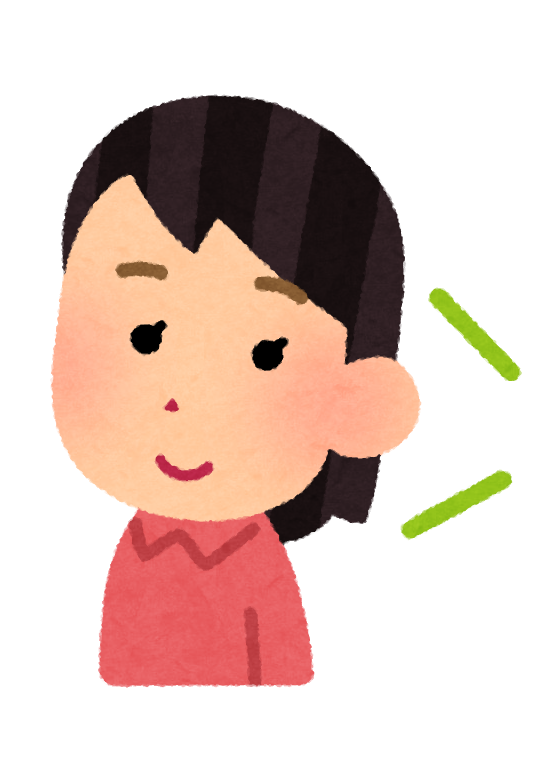
\includegraphics[width=3cm]{study_gogaku_woman_listning.png}
  \vspace{-1.4\baselineskip}
\end{wrapfigure}
Ich sage zwei Ketten aus \textbf{denselben vier Wörtern}. Sag mir, was sich ändert.

\begin{center}
\begin{tabular}{@{}ll@{}}
(a) & \jterm{父}{ちち}の\jterm{大切}{たいせつ}な\jterm{古}{ふる}い本 \\[4pt]
(b) & \jterm{大切}{たいせつ}な\jterm{父}{ちち}の\jterm{古}{ふる}い本 \\
\end{tabular}
\end{center}

\textbf{Wer ist in (b) wichtig — der Vater oder das Buch?}

Dann drehen wir's mit anderen Wörtern durch:

\begin{center}
\begin{tabular}{@{}l@{}}
\jterm{母}{はは}の上手な丸い\jterm{字}{じ} ／ 上手な\jterm{母}{はは}の丸い\jterm{字}{じ} \\[4pt]
\jterm{友人}{ゆうじん}の\jterm{大切}{たいせつ}な小さい犬 ／ \jterm{大切}{たいせつ}な\jterm{友人}{ゆうじん}の小さい犬 \\
\end{tabular}
\end{center}

\begin{merke}
\textbf{Das Ohr merkt es schneller als das Auge.} の sucht sich das nächste Nomen —
und wenn eins danebensteht, nimmt es das.
\end{merke}

\section{Verneint stapeln \textcolor{explizit}{$\bigstar$}}

\begin{center}
\begin{tabular}{@{}ll@{}}
A：\jterm{大切}{たいせつ}な本？ & B：\jterm{大切}{たいせつ}じゃない本。\\[4pt]
A：大きい犬？ & B：大きくない犬。\\[4pt]
A：出る人？ & B：出ない人。\\
\end{tabular}
\end{center}

\begin{merke}
Beim ersten Paar passiert was, das du erklären können solltest:
\textbf{Wo ist das な hin?}
\end{merke}

\section{Beschreib mir was}

Such dir einen Gegenstand im Raum aus und sag mir drei Sachen dazu — aber benutz
\textbf{beide Gruppen}, einmal \expl{} und einmal \impl{}.

\begin{center}
本。\jterm{父}{ちち}の本。\jterm{古}{ふる}い。\jterm{大切}{たいせつ}じゃない。
\end{center}

Wenn dir auffällt, dass das noch keine richtigen Sätze sind: stimmt. Dafür fehlen
は und die Verb-Vergangenheit. Kommt beides.

\end{document}
